\subsection{Lorenz System}
\subsubsection{Problem Formulation}
We remind the reader of the Lorenz ODE system given in equation \ref{eq:lorenz}, which we repeat here:
\begin{equation*}
\begin{aligned}
    \dot{x} &= 10y - 10x, \\
    \dot{y} &= 28x - xz - y, \\
    \dot{z} &= xy - \frac 8 3 z,
\end{aligned}
\end{equation*}
We attempt to reproduce the results of \textcite{Champion_2019}.

Hence, given the generated high-dimensional data discussed in \ref{sec:method}, we consider an encoder with layer widths widths $[128, 64, 32, 3]$, and a decoder with layer widths $[3, 32, 64, 128]$, where 128 is the dimension of our high-dimensional data, and 3 is the dimension of our latent-space. 
We consider a loss formulation with regularization, running $10,000$ initial epochs with regularization and sequential least squares thresholding, before running an additional $1,000$ simulations without regularization. 
To optimize our SINDy Autoencoder, we apply \textsc{ADAM} with a learning rate of $10^{-3}$. 
Further specifics about the training parameters can be found in \autoref{table:lorenz}. 

\begin{table}
\caption{Specifications and hyperparameters used for training our Lorenz system.}
\centering
\begin{tabular}{|l|r|}\hline
    Parameter & Value \\
    \hline
    n & $128$\\
    d & $3$\\
    \text{training samples} & $5.12 \times 10^5$ \\
    batch size & $8000$ \\
    activation function & sigmoid \\
    encoder layers widths & [64, 32]\\
    decoder layer width & [32, 64]\\
    learning rate & $10^{-3}$\\
    SINDy library polynomial order & 3\\
    SINDy library include sines & no\\
    $\lambda_1$ & $10^{-4}$\\
    $\lambda_2$ & $0$ \\
    $\lambda_3$ & $10^{-5}$\\
    thresholding frequency & $500$\\
    thresholding value & $0.1$\\
    \hline
\end{tabular}
\label{table:lorenz}
\end{table}
Using these parameters, we trained 10 models with different random seeds, comparing their results. 

\subsubsection{Results}



\begin{figure}[htbp]
    \centering
    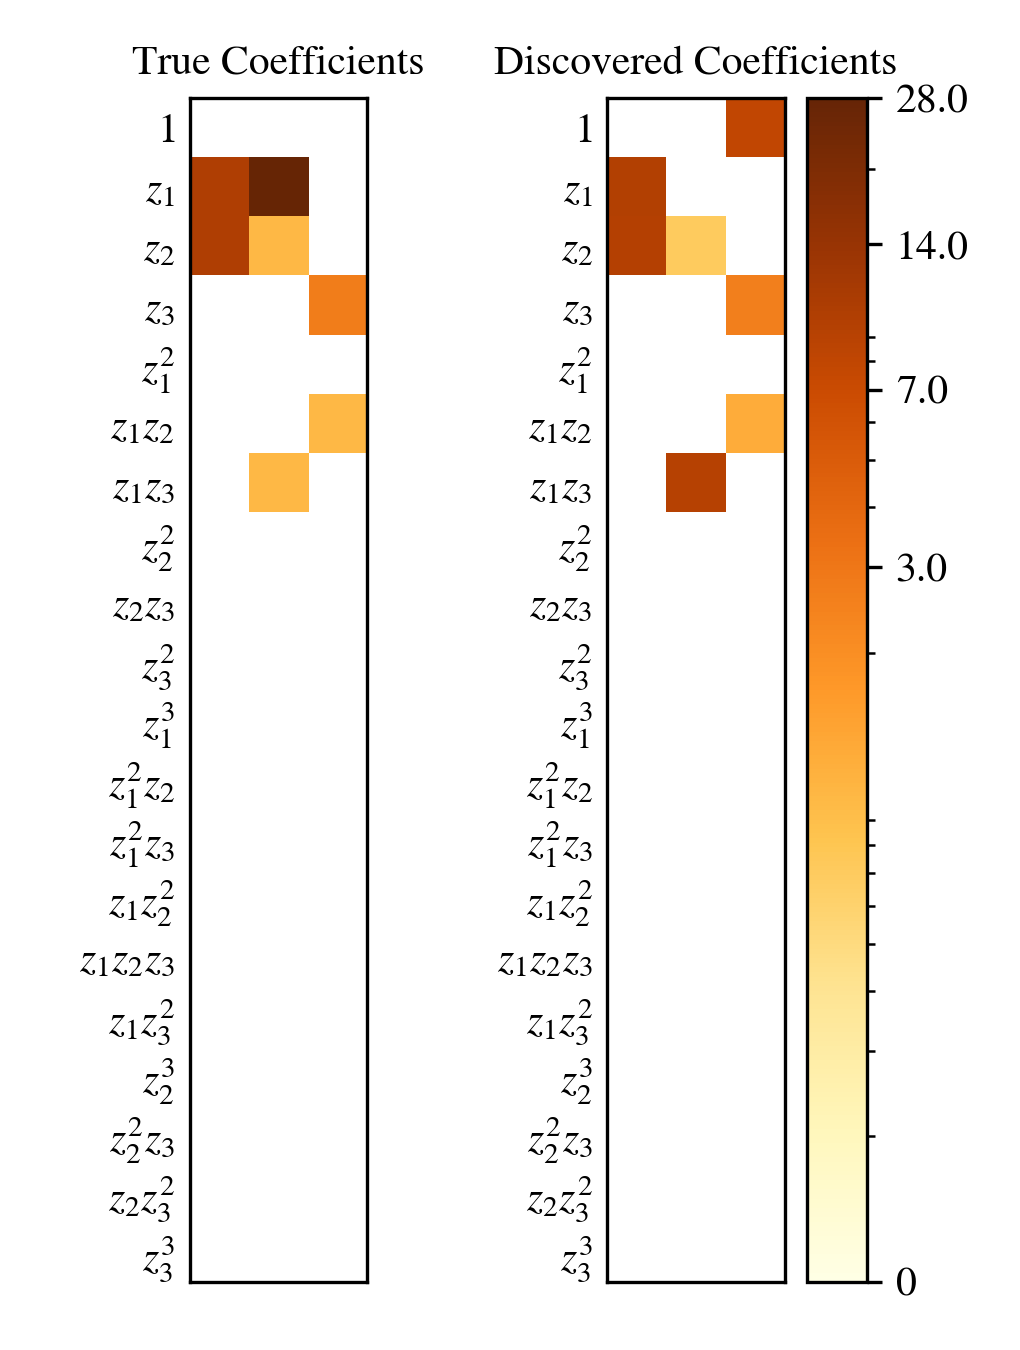
\includegraphics[width=0.45\textwidth]{project_2/images/xi_plot_lorenz.png}
    \vspace{-4mm}
    \caption{\textbf{Comparison of True and Discovered Coefficients for the Lorenz System:} This figure displays a side-by-side comparison of the true coefficients (left) against those discovered by the framework (right) in the Xi matrix. Each coefficient's magnitude is visualized by the color intensity. The discovered coefficients closely align with the true coefficients, except for slight variations in a few terms.}
    \label{fig:xi_plot_lorenz}
\end{figure}
\begin{figure*}[t]
\centering
\begin{minipage}[b]{.45\textwidth}
\centering
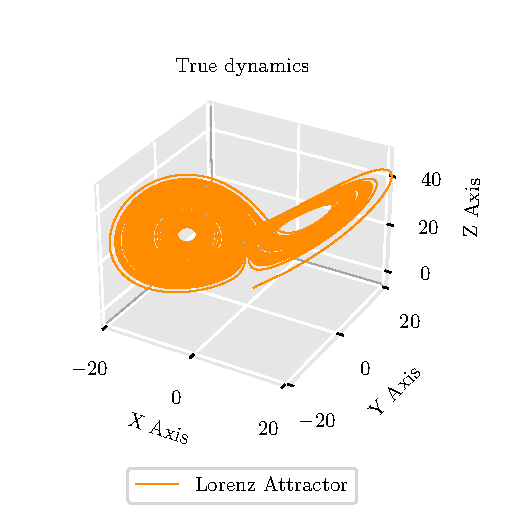
\includegraphics[width=\textwidth]{project_2/images/lorenz_true_dynamics.pdf}
\caption{\textbf{True Lorenz dynamics:} This figure shows the true Lorenz dynamics for the initial conditions [1, 1, 1] found using the true ODE system seen in \autoref{eq:lorenz}.}
\label{fig:lorenz_true_dynamics}
\end{minipage}\qquad\quad
\begin{minipage}[b]{.45\textwidth}
\centering
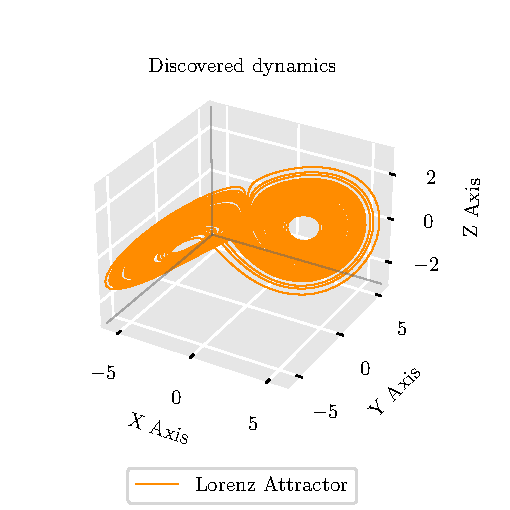
\includegraphics[width=\textwidth]{project_2/images/lorenz_discovered_dynamics.pdf}
\caption{\textbf{Discovered Lorenz dynamics:} This figure shows the discovered Lorenz dynamics for the initial conditions [1, 1, 1] found by the autoencoder SINDy framework.}
\label{fig:lorenz_discovered_dynamics}
\end{minipage}
\end{figure*}

\begin{figure*}[t]
\centering
\begin{minipage}[b]{.45\textwidth}
\centering
    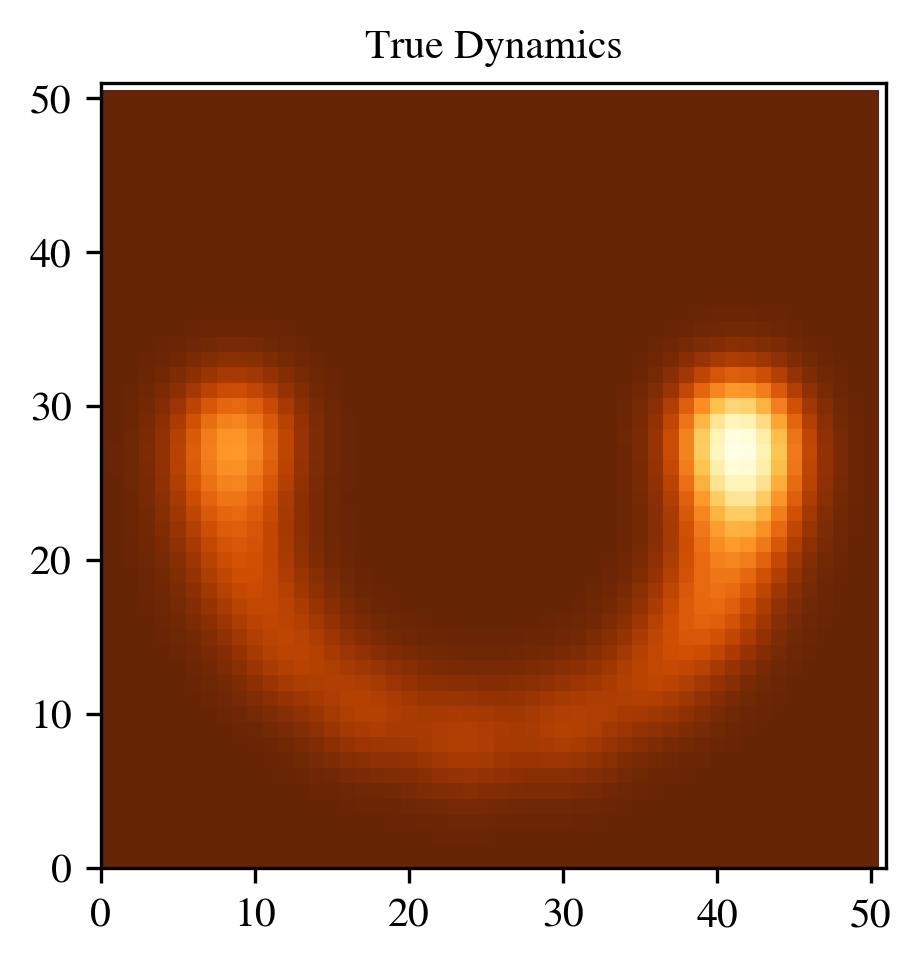
\includegraphics[width=0.8\textwidth]{project_2/images/true_heatmap_pendulum.png}
    \caption{\textbf{True pendulum dynamics:} Heat map of the true pendulum dynamics with initial conditions $\theta=1.5,\ \dot{\theta}=0.8$.}
    \label{fig:true_heatmap_pendulum}
\end{minipage}\qquad\quad
\begin{minipage}[b]{.45\textwidth}
\centering
    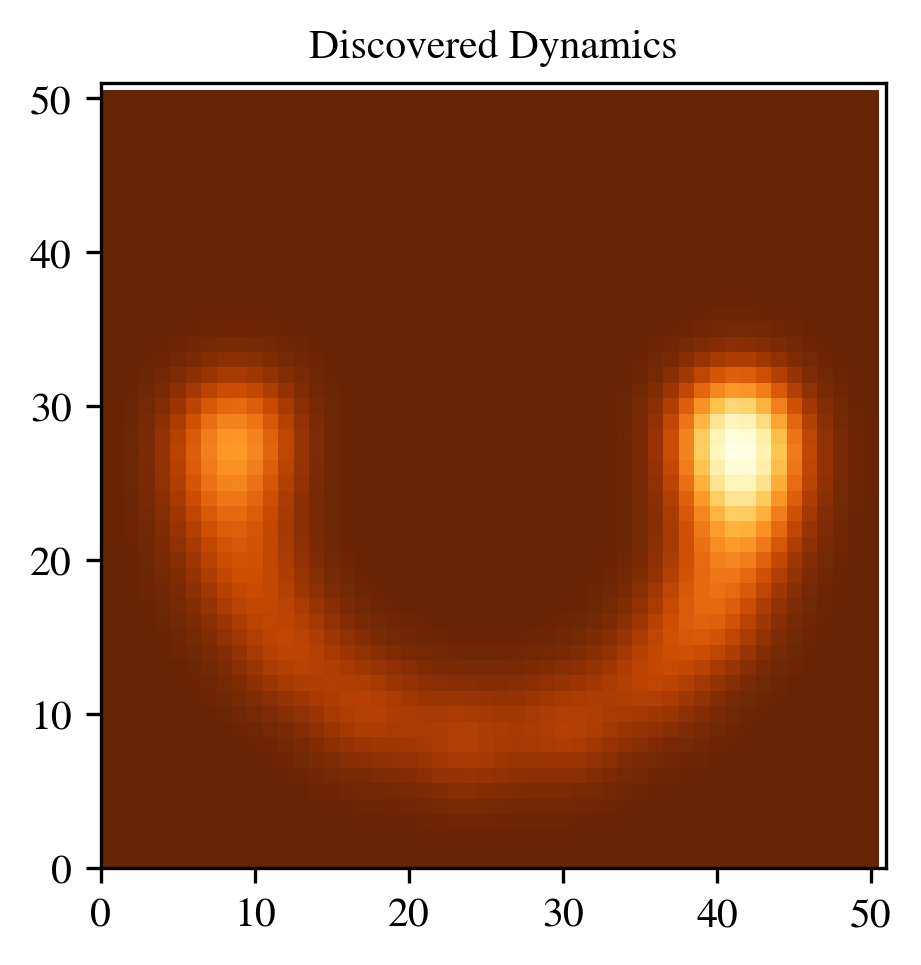
\includegraphics[width=0.8\textwidth]{project_2/images/discovered_heatmap_pendulum.png}
    \caption{\textbf{True pendulum dynamics:} Heat map of the discovered pendulum dynamics with initial conditions $\theta=1.5,\ \dot{\theta}=0.8$.}
    \label{fig:discovered_heatmap_pendulum}
\end{minipage}
\end{figure*}
Given our knowledge of the Lorenz system, but also the fact that we desire parsimonious and sparse models, we choose to investigate our sparsest model. 

The loss evolution of the sparsest model can be seen in \autoref{fig:lorenz_loss}.
We note that the sudden drop  in validation loss at 10,000 epochs corresponds with the regularization cutoff, where the model is trained without regularization. 
Moreover, we note that the instability of the loss after reaching a value of $10^{-5}$ might be due to the fact that we, like \textcite{Champion_2019} use a constant learning rate, perhaps causing \textsc{Adam} to overcorrect at each gradient step. 
A learning rate scheduler might have helped alleviate this phenomenon. 

\begin{figure}
    \centering
    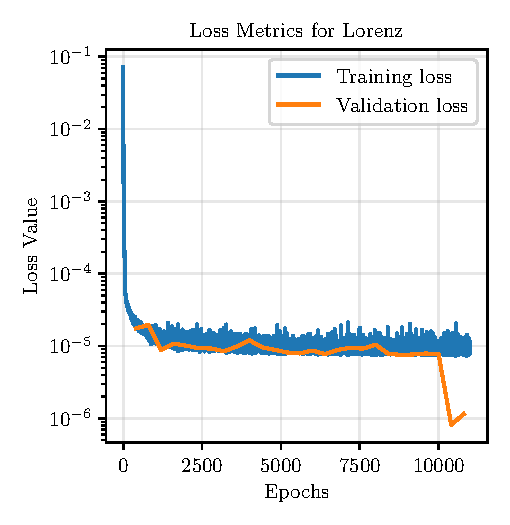
\includegraphics[width=0.48\textwidth]{project_2/images/Loss Metrics for Lorenz.pdf}
    \vspace{-8mm}
    \caption{\textbf{Loss metrics for Lorenz model training over epochs:} This figure shows the training and validation loss for the lorenz dynamics discovery. We see that the training loss has converged, but that the validation loss has a downwards spike at the at the end of the training session.}
    \label{fig:lorenz_loss}
\end{figure}





\subsection{Non-linear Pendulum}
\subsubsection{Problem Formulation}
We again remind the reader of the non-linear pendulum equation given in \ref{eq:pendel}, which is repeated below. 
\begin{equation*}
    \ddot{z} = -\sin(z).
\end{equation*}
Like with the lorenz system, we attempt to reproduce the results of \cite{Champion_2019}. 
The setup specifics for the model are given in \autoref{table:pendulum}. Note that we apply a much smaller batch size 250 compared to Kathleen's 1024. This was primarily done due to excessive memory pressure during our simulations. In addition, the non-linear pendulum is trained with \verb|JAX|'s default x32-bit floats instead of x64-bit floats for the same reason. 

Also note that since the equation is second order, the SINDy library includes both $z$ and $\dot{z}$ terms, alongside their respective sines. 
\begin{table}
\caption{Specifications and hyperparameters used for training the non-linear pendulum.}
\centering
\begin{tabular}{|l|r|}\hline
    Parameter & Value \\
    \hline
    n & $2601$\\
    d & $1$\\
    \text{training samples} & $5 \times 10^4$ \\
    batch size & $250$ \\
    activation function & sigmoid \\
    encoder layers widths & [128, 64, 32]\\
    decoder layer width & [32, 64, 128]\\
    learning rate & $10^{-4}$\\
    SINDy library polynomial order & 3\\
    SINDy library include sines & yes\\
    $\lambda_1$ & $5 \times 10^{-4}$\\
    $\lambda_2$ & $5 \times 10^{-5}$ \\
    $\lambda_3$ & $10^{-5}$\\
    thresholding frequency & $500$\\
    thresholding value & $0.1$\\
    \hline
\end{tabular}
\label{table:pendulum}
\end{table}

Using these parameters, we trained 9 models with different random seeds, comparing their results. 

\subsubsection{Results}
Out of the 9 trained models 5 of the models converged towards the correct single sine term, whereas 4 of the models included an additional linear term. 
The loss evolution of one of the 5 successful models is displayed in \autoref{fig:lorenz_loss}.

\begin{figure}[!htbp]
    \centering
    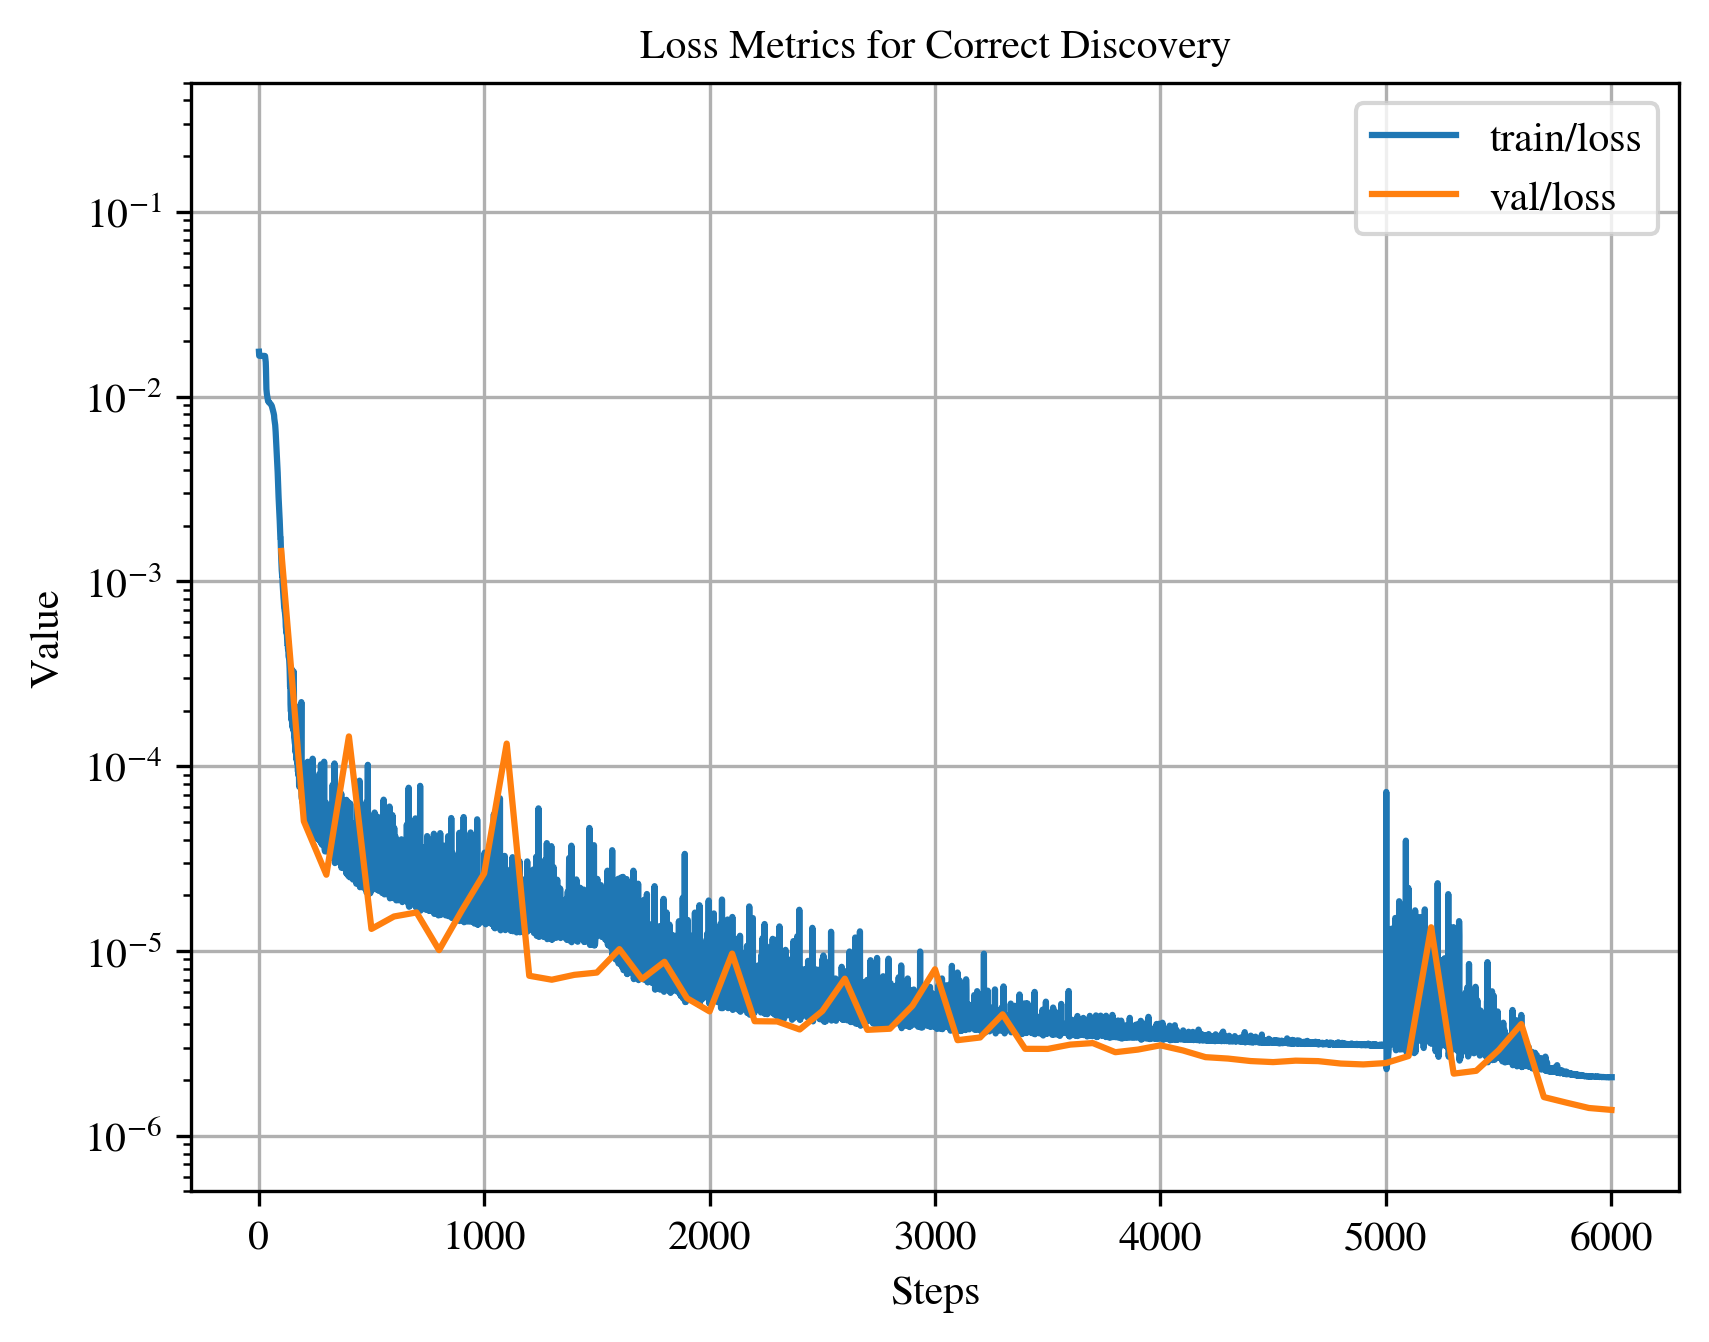
\includegraphics[width=0.48\textwidth]{project_2/images/Loss Metrics for Pendulum.png}
    \vspace{-8mm}
    \caption{\textbf{Loss metrics for pendulum model training over epochs:} This plot depicts both training and validation losses for the non-linear pendulum. At epoch 5000, a significant modification in the training process is implemented by removing the \(\text{L}_1\) regularization, from the loss function. This adjustment allows coefficients that had not converged to zero to potentially increase, as observed by the notable spike in loss values. This strategic change is aimed at enhancing model adaptability by reevaluating the significance of previously diminished coefficients.}
    \label{fig:lorenz_loss}
\end{figure}

The correct models accurately identified the dynamics governing the pendulum's motion. 
The discovered coefficients highlight that the model found the single nonlinear term $\sin (z)$, which is what gives the pendulum its periodic nature. 
The true and discovered latent dynamics 

%All other terms have zero coefficients, correctly indicating that they do not contribute to the system dynamics. 
